\documentclass[a4paper]{article}
\usepackage{amsmath,amssymb,caption,float,graphicx,minted,xcolor}
\usepackage[utf8]{inputenc}
\usepackage[english]{babel}
\usepackage[backend=bibtex]{biblatex}
\addbibresource{Lab2.bib}
\captionsetup[figure]{labelsep=period}
\definecolor{bg}{rgb}{0.95,0.95,0.95}
\renewcommand\thesection{\arabic{section}}
\usemintedstyle{emacs}
\begin{document}
\begin{center}
    \huge
    \textbf{VE482\\Introduction to Operating Systems\\}
    \Large
    \vspace{15pt}
    \uppercase{\textbf{Lab 2}}\\
    \large
    \vspace{5pt}\today\\
    \vspace{5pt}
    Yihua Liu 518021910998
    \vspace{5pt}
    \rule[-5pt]{.97\linewidth}{0.05em}
\end{center}
\section{Minix 3}
\begin{itemize}
    \item In Minix 3, how to manage software, i.e. install, remove, update, etc.? \cite{pkgin}
    \begin{itemize}
        \item Install: \texttt{pkgin install foo}
        \item Remove: \texttt{pkgin remove foo}
        \item Update: \texttt{pkgin update}
        \item Upgrade: \texttt{pkgin upgrade}
        \item Upgrade all: \texttt{pkgin full-upgrade}
        \item List available packages: \texttt{pkgin avail}
        \item List installed packages: \texttt{pkgin list}
        \item Remove orphan dependencies: \texttt{pkgin autoremove}
        \item Delete downloaded packages from the cache directory: \texttt{pkgin clean}
    \end{itemize}
    \item What is the purpose of the commands \texttt{ifconfig}, \texttt{adduser}, and \texttt{passwd}?
    \begin{itemize}
        \item \texttt{ifconfig} - configure a TCP/IP device: initializes a TCP/IP setting the IP address and/or netmask. It will report the address and netmask set \cite{ifconfig}.
        \item \texttt{adduser} - add a user to the system \cite{useradd}: creating and populating a home directory if necessary. The arguments to adduser are the user name, the group name, and the user's home directory \cite{adduser}.
        \item \texttt{passwd} - modify a user's password: changes the user's password \cite{passwd}.
    \end{itemize}
\end{itemize}
\section{Working on a remote server}
\begin{itemize}
    \item Setup an SSH server on Minix 3. From Linux (using ssh) or Windows (using Putty) log into Minix 3. Note: the network need to be properly setup on the Virtual Machine (VM).\\
    On Minix 3:
    \begin{minted}[frame=single,bgcolor=bg,breaklines,linenos]{bash}
        pkgin update
        pkgin install openssh
        user add -m -g users yihua  # optional, "users" is the group name (the same as "other")
    \end{minted}
    On WSL Ubuntu:
    \begin{minted}[frame=single,bgcolor=bg,breaklines,linenos]{bash}
        sudo apt update
        sudo apt upgrade
        sudo apt install openssh-client
        ssh root@192.168.36.136  # default port is 22
    \end{minted}
    On PowerShell Core 7:
    \begin{minted}[frame=single,bgcolor=bg,breaklines,linenos]{bash}
        ssh root@192.168.36.136  # default port is 22
    \end{minted}
    \item What is the default SSH port? Change this port for port 2222. Log into Minix 3 using this new SSH server setup.
    The default SSH port is 22. To change this port for port 2222, on Minix 3:
    \begin{minted}[frame=single,bgcolor=bg,breaklines,linenos]{bash}
        vi /usr/pkg/etc/ssh/sshd_config  # delete # and change the line to Port 2222
    \end{minted}
    \begin{figure}[H]
        \centering
        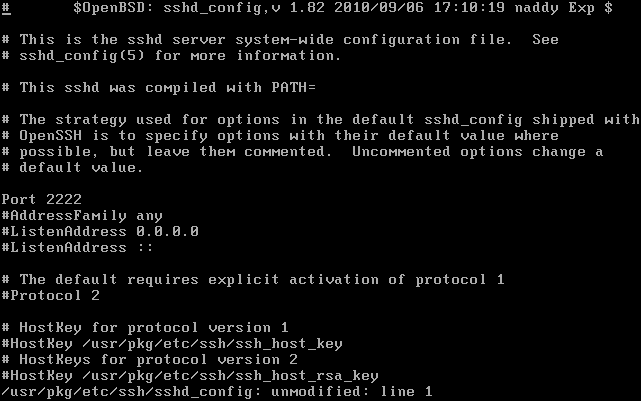
\includegraphics[width=0.8\textwidth]{1.png}
        \caption{Screenshot of \texttt{sshd\_config} on Minix 3.2.1.}
    \end{figure}
    On WSL Ubuntu or PowerShell Core 7:
    \begin{minted}[frame=single,bgcolor=bg,breaklines,linenos]{bash}
        ssh root@192.168.36.136 -p 2222
    \end{minted}
    \begin{figure}[H]
        \centering
        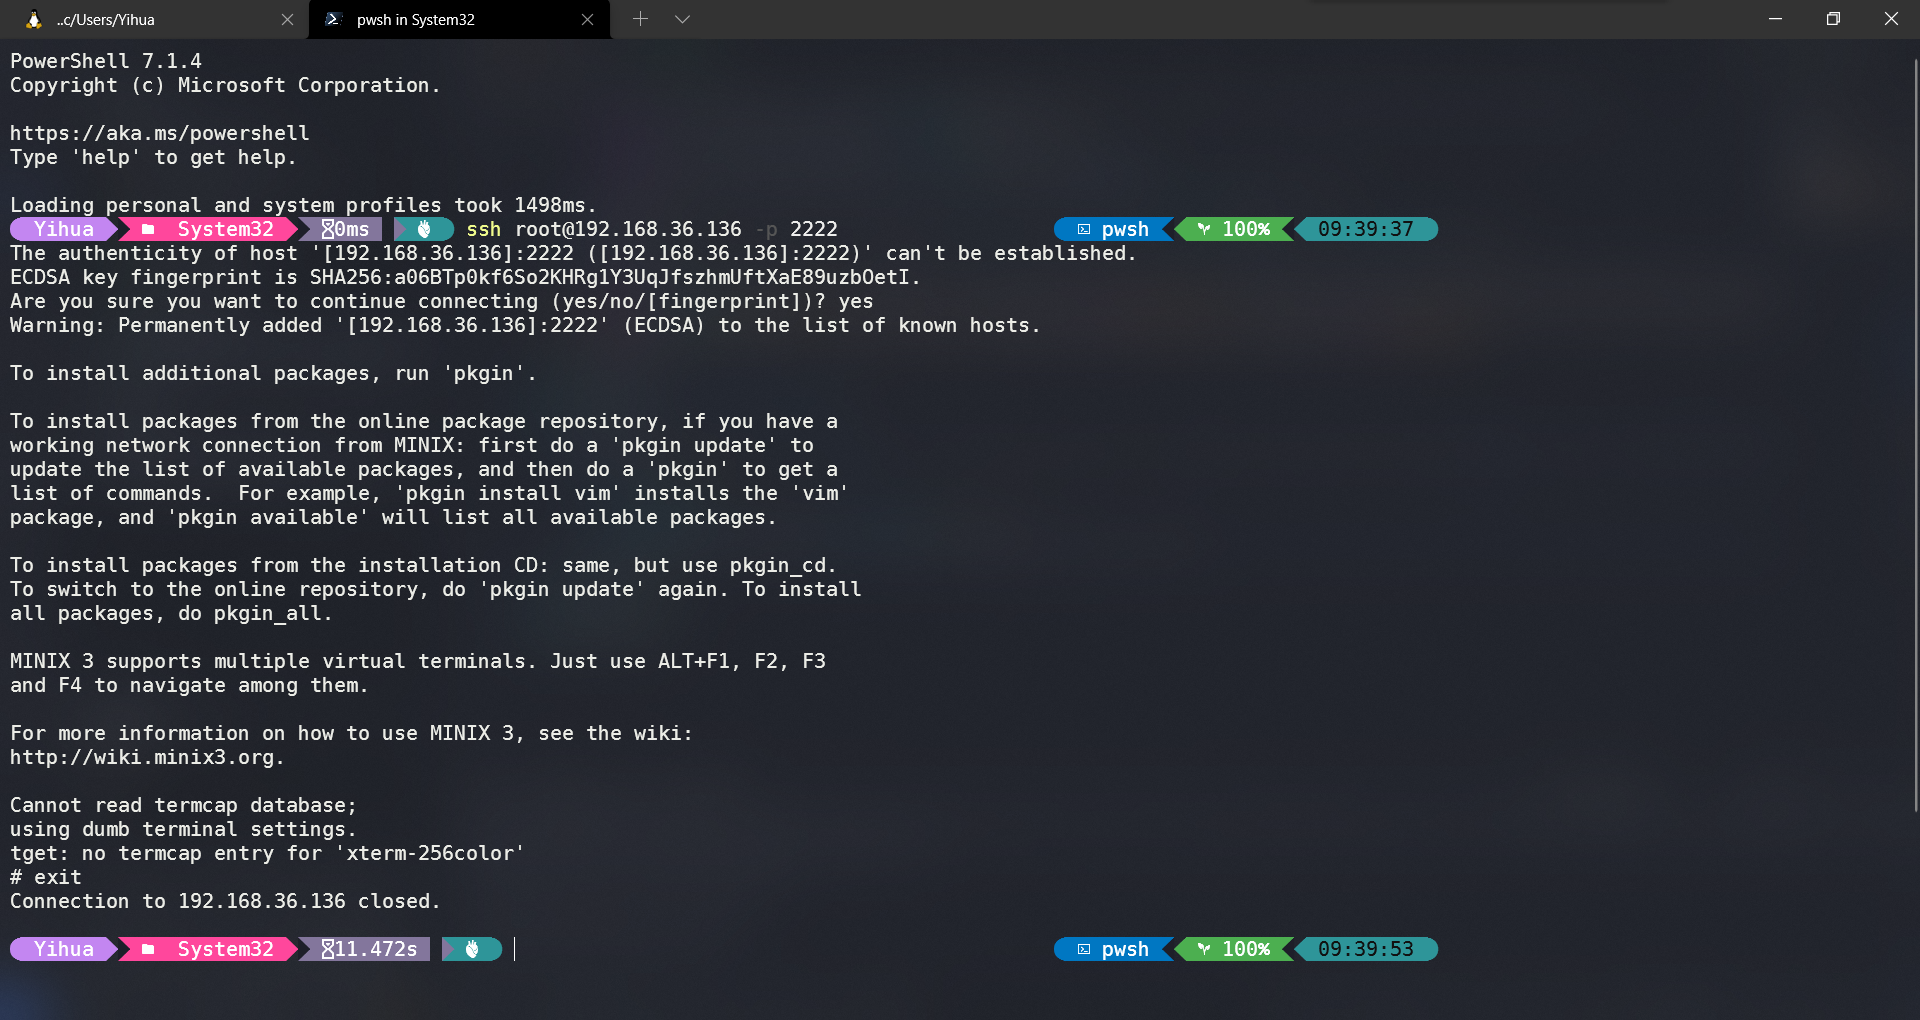
\includegraphics[width=0.8\textwidth]{2.png}
        \caption{Screenshot of PowerShell Core 7 logging into Minix 3.}
    \end{figure}
    \item List and explain the role of each the file in the \texttt{\$HOME/.ssh} directory. In \texttt{\$HOME/.ssh/config}, create an entry for Minix 3.
    \begin{itemize}
        \item authorized\_keys: a list of public SSH keys that is used to match users' private SSH keys to establish connections
        \item config: SSH client configuration
        \item id\_rsa: private SSH key
        \item id\_rsa: public SSH key
        \item known\_hosts: a list of hosts that users have logged into
    \end{itemize}
    \begin{figure}[H]
        \centering
        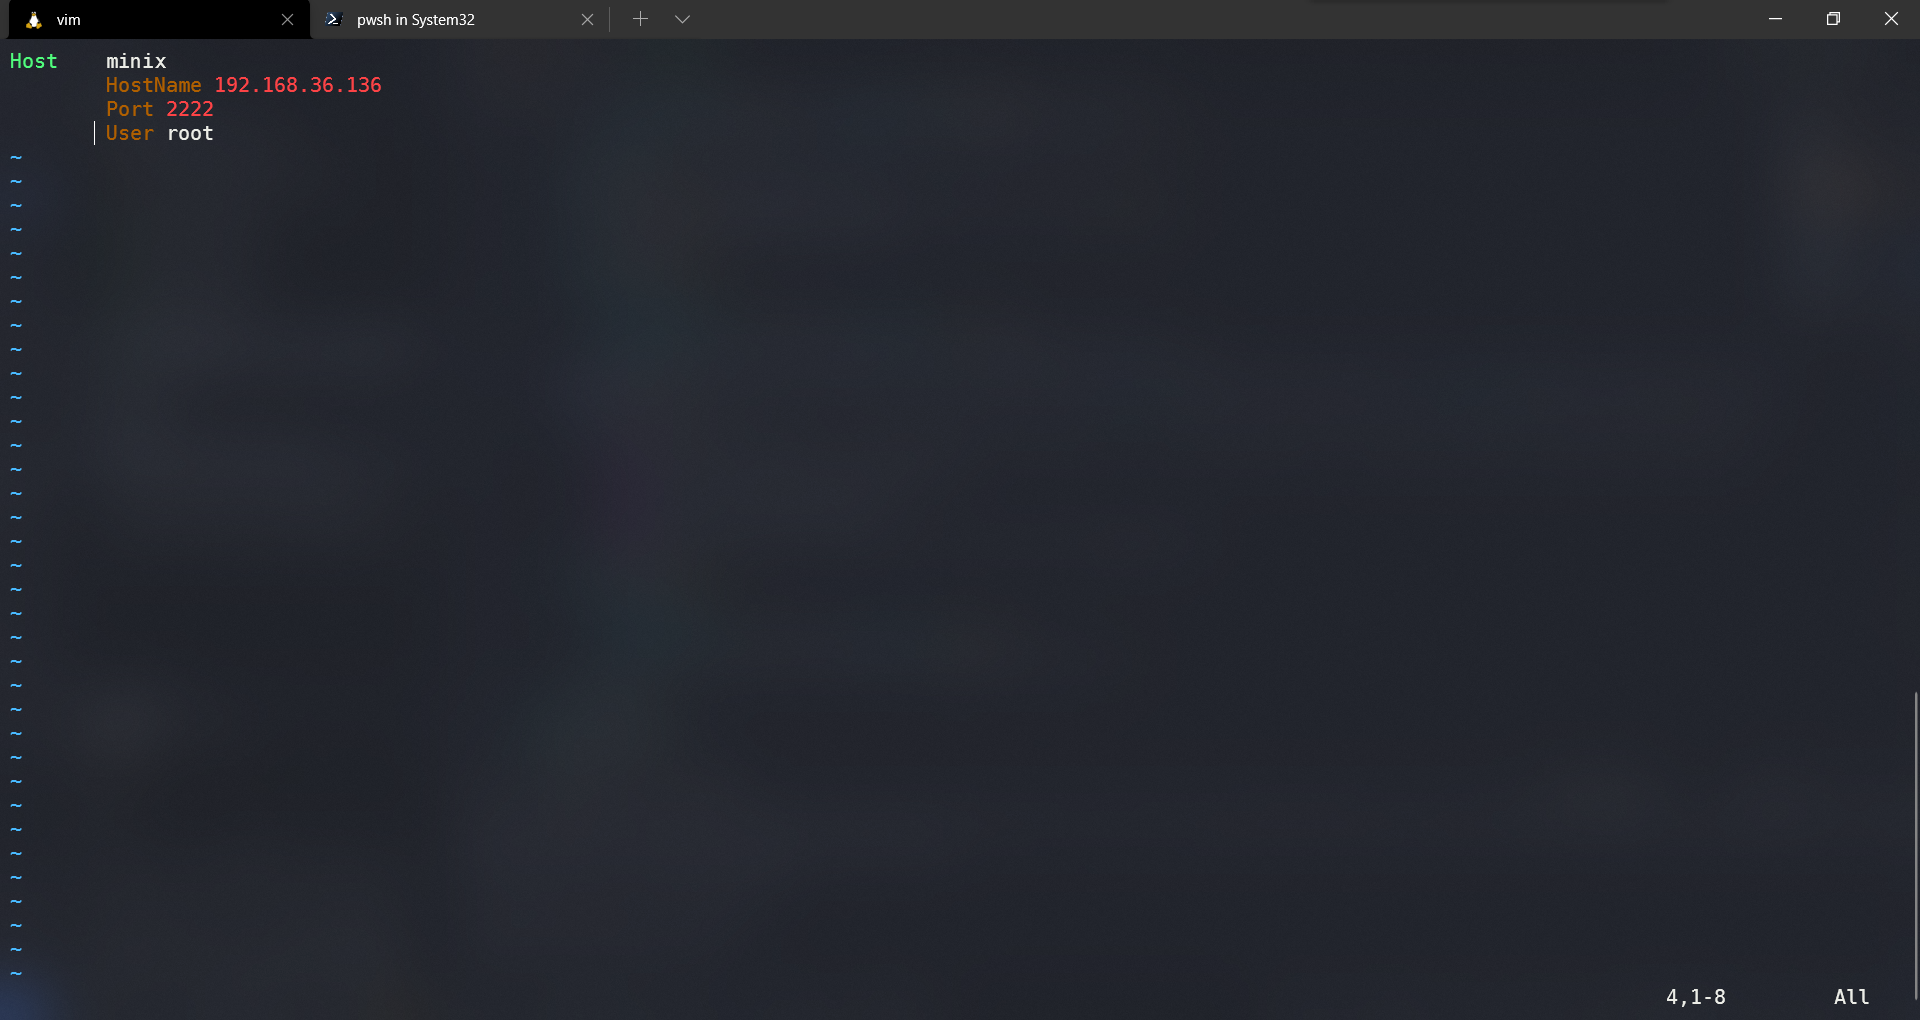
\includegraphics[width=0.8\textwidth]{4.png}
        \caption{Screenshot of \texttt{~/.ssh/config} creating an entry for Minix 3.}
    \end{figure}
    \item Briefly explain how key-only authentication works in SSH. Generate a key-pair on the host system and use it to log into Minix 3 without a password.
    Key-only authentication works in SSH is based on asymmetric cryptography. Given user-generated SSH key pairs (a private SSH key and a public SSH key) done by ssh-keygen, the public key will be sent to the server by ssh-copy-id. Then, the server will store the public key, marks it as authorized, and allows access to anyone who can prove they have the corresponds private key \cite{ssh}.\\
    On WSL Ubuntu:
    \begin{minted}[frame=single,bgcolor=bg,breaklines,linenos]{bash}
        vim ~/.ssh/config  # add minix host
        ssh minix
    \end{minted}
    \texttt{$\sim$/.ssh/config}:
    \begin{minted}[frame=single,bgcolor=bg,breaklines,linenos]{text}
        Host    minix
                HostName 192.168.130.138
                Port 2222
                User root
    \end{minted}
    \begin{figure}[H]
        \centering
        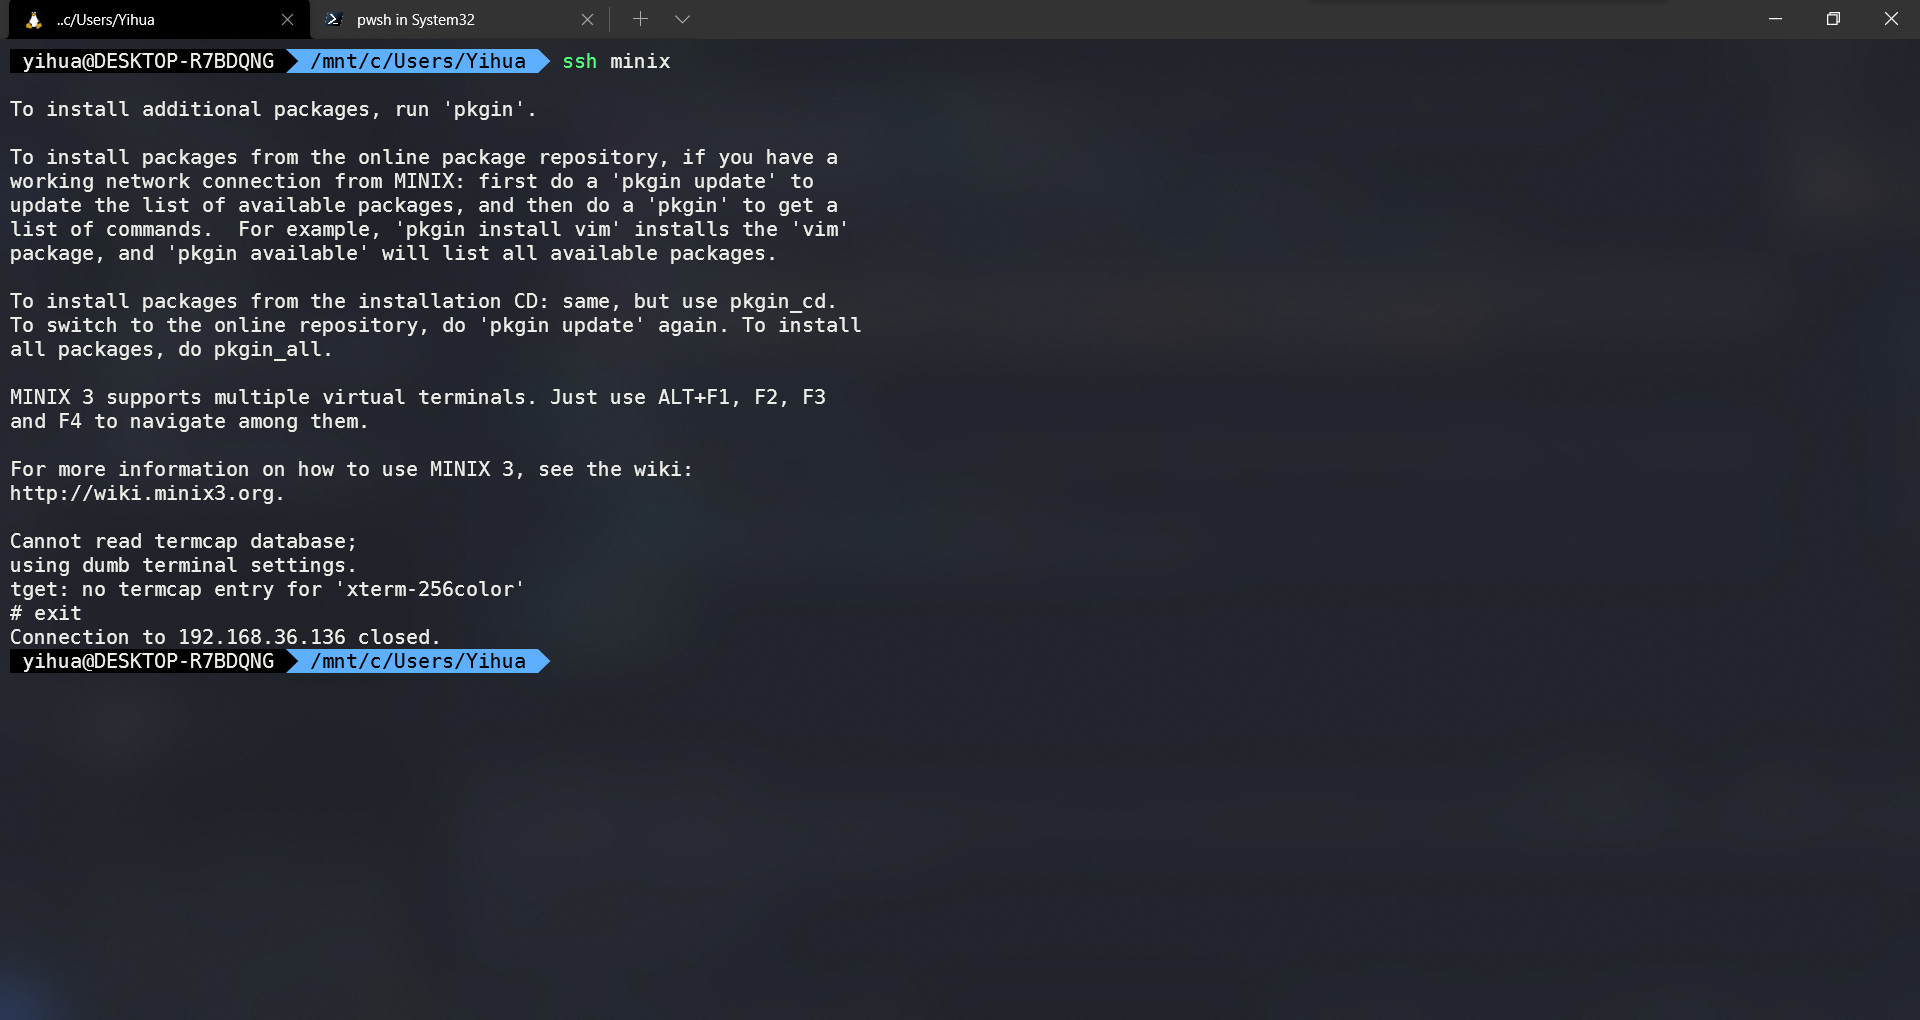
\includegraphics[width=0.8\textwidth]{3.png}
        \caption{Screenshot of WSL Ubuntu logging into Minix 3.}
    \end{figure}
    \item On Canvas, submit your public key in a \textit{separate file}. Name it “student-id.pub”, e.g. “5143709219.pub”. This public key will be used to grant you access to the VE482 course server. Note: always remember that the private keys should remain \textit{private}, and as such should never be disclosed.
\end{itemize}
\section{Basic git}
\begin{itemize}
    \item Setup git on your computer, we will use it for the rest of the semester.
    \item Search the use of the following \texttt{git} commands \cite{git}:
    \begin{itemize}
        \item \texttt{help} - Display help information about Git.
        \item \texttt{branch} - List, create, or delete branches.
        \item \texttt{merge} -  Join two or more development histories together: Incorporates changes from the named commits (since the time their histories diverged from the current branch) into the current branch.
        \item \texttt{tag} - Create, list, delete or verify a tag object signed with GPG.
        \item \texttt{commit} - Record changes to the repository: Create a new commit containing the current contents of the index and the given log message describing the changes.
        \item \texttt{init} - Create an empty Git repository or reinitialize an existing one: This command creates an empty Git repository - basically a \texttt{.git} directory with subdirectories for \texttt{objects}, \texttt{refs/heads}, \texttt{refs/tags}, and template files.
        \item \texttt{push} - Update remote refs along with associated objects: Updates remote refs using local refs, while sending objects necessary to complete the given refs.
        \item \texttt{add} - Add file contents to the index: This command updates the index using the current content found in the working tree, to prepare the content staged for the next commit.
        \item \texttt{log} - Show commit logs: Shows the commit logs. List commits that are reachable by following the \texttt{parent} links from the given commit(s), but exclude commits that are reachable from the one(s) given with a \^{} in front of them.
        \item \texttt{clone} - Clone a repository into a new directory: Clones a repository into a newly created directory, creates remote-tracking branches for each branch in the cloned repository (visible using \texttt{git branch --remotes}), and creates and checks out an initial branch that is forked from the cloned repository’s currently active branch.
        \item \texttt{checkout} - Switch branches or restore working tree files: Updates files in the working tree to match the version in the index or the specified tree.
        \item \texttt{pull} - Fetch from and integrate with another repository or a local branch: Incorporates changes from a remote repository into the current branch.
        \item \texttt{diff} - Show changes between commits, commit and working tree, etc: Show changes between the working tree and the index or a tree, changes between the index and a tree, changes between two trees, changes resulting from a merge, changes between two blob objects, or changes between two files on disk.
        \item \texttt{fetch} - Download objects and refs from another repository: Fetch branches and/or tags (collectively, "refs") from one or more other repositories, along with the objects necessary to complete their histories.
        \item \texttt{reset} - Reset current HEAD to the specified state.
    \end{itemize}
    \item Setup your \texttt{git} repository on the VE482 server.
\end{itemize}
\printbibliography
\end{document}